\subsection{Region Three Construction (Special Considerations)}

The R3 chambers were designed and constructed at Jefferson Laboratory.  
They have the same shape as the other chambers but are larger,
4~m on a side, so the wires are as long as 4~m.
To reduce the gravitational sag of these very long wires we
strung wires with lengths between 0.6 and 0.8 of the maximum length
at 30~g and the longest wires with lengths greater than 0.8 of maximum 
at 40~g, twice the nominal tension of 20~g.

%%%%%%%%%%%%%%%%%%% Figure : Region Three Cross Section %%%%%%%%%%%%%%%%%%
\begin{figure}[htpb]   
\vspace{4.6cm}
\begin{picture}(35,35)
\put(35,-5)
{\hbox{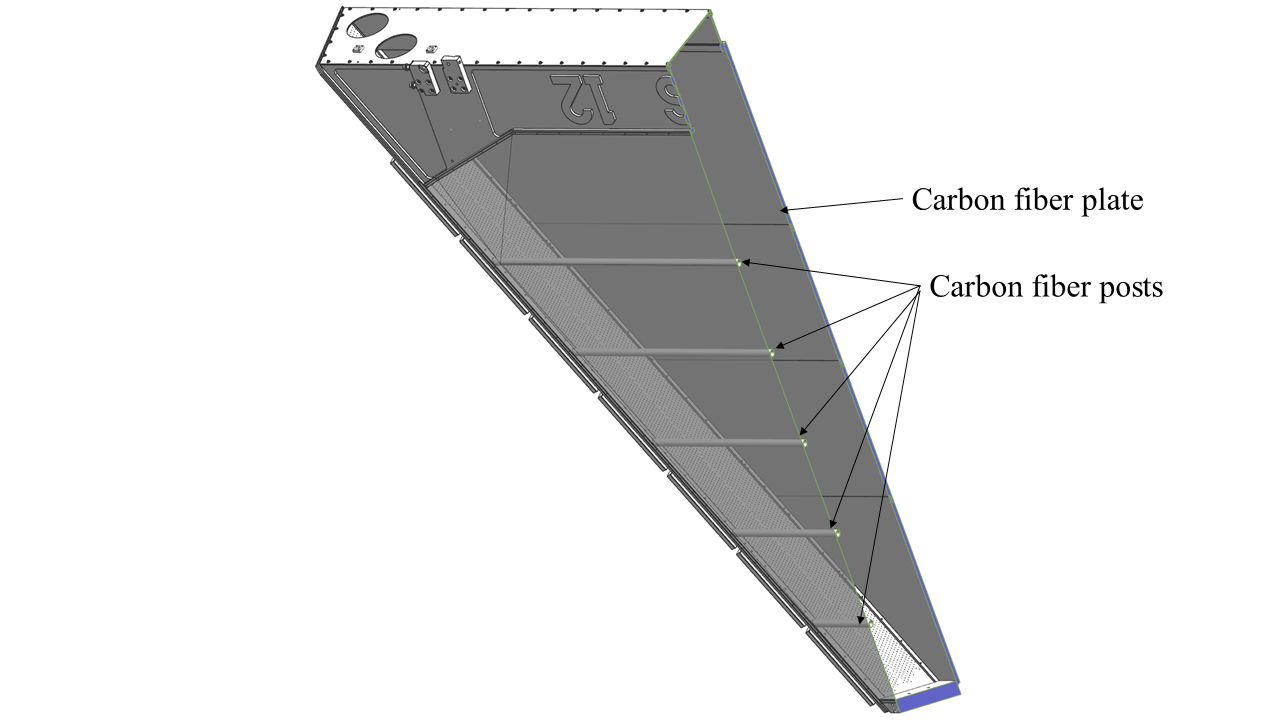
\includegraphics[width=0.8\columnwidth,natwidth=610,natheight=642]{img/dcr3-midplane-cut.png}}}
\end{picture}
\caption{\small{Assembly drawing of a R3 chamber showing the component parts and highlighting the
    carbon-fiber tubes at the entrance face and
the carbon-foam composite plate at the exit, which supported the endplates
against the wire tension.}}
\label{dcr3-midplane-cut}
\end{figure}   
%%%%%%%%%%%%%%%%%%%%%%%%%%%%%%%%%%%%%%%%%%%%%%%%%%%%%%%%%%

Because these are the last of the tracking chambers, multiple scattering
at the chamber entrance is less important than multiple scattering that
occurs at a R1 or a R2 chamber.  This allowed us to 
build a chamber in which the endplates were not supported only on
their ends. See Fig.~\ref{dcr3-midplane-cut} for a depiction of the R3 box assembly. 

At the entrance face we included 7 thin-walled carbon
fiber tubes to span the gap and hold the endplates apart.  At the
exit face the endplates were coupled to a triangular carbon-foam-carbon
composite plate that similarly supported the wire tension.
